\documentclass[11pt,a4paper]{article}

\usepackage[utf8]{inputenc}
\usepackage{xeCJK}
\usepackage{geometry}
\usepackage{hyperref}
\usepackage{titlesec}
\usepackage{enumitem}
\usepackage{xcolor}
\usepackage{graphicx}

\geometry{left=1.5cm, right=1.5cm, top=1.8cm, bottom=1.8cm}
\pagestyle{empty}

\definecolor{darkblue}{RGB}{0, 0, 139}
\hypersetup{colorlinks=true, urlcolor=darkblue}

\titleformat{\section}{\large\bfseries}{}{0em}{}[\titlerule]
\titlespacing{\section}{0pt}{12pt}{8pt}

\begin{document}

% 姓名与照片区域
\noindent
\begin{minipage}[c]{0.75\textwidth}
    {\huge \bfseries 何奇正 (Qizheng He)} \\
    \vspace{6pt}
    (+86) 130-6656-5618 |
    微信：qzhbio |
    \href{mailto:heqz9923@mails.jlu.edu.cn}{heqz9923@mails.jlu.edu.cn} |
    男 \\
    ORCID: \href{https://orcid.org/0009-0009-1002-9556}{0009-0009-1002-9556} | 
    \href{https://scholar.google.com/citations?user=l9sH920AAAAJ}{Google Scholar} \\
    \vspace{4pt}
    吉林大学 · 生命科学学院 · 唐敖庆理科试验班
\end{minipage}%
\begin{minipage}[c]{0.25\textwidth}
    \raggedleft
    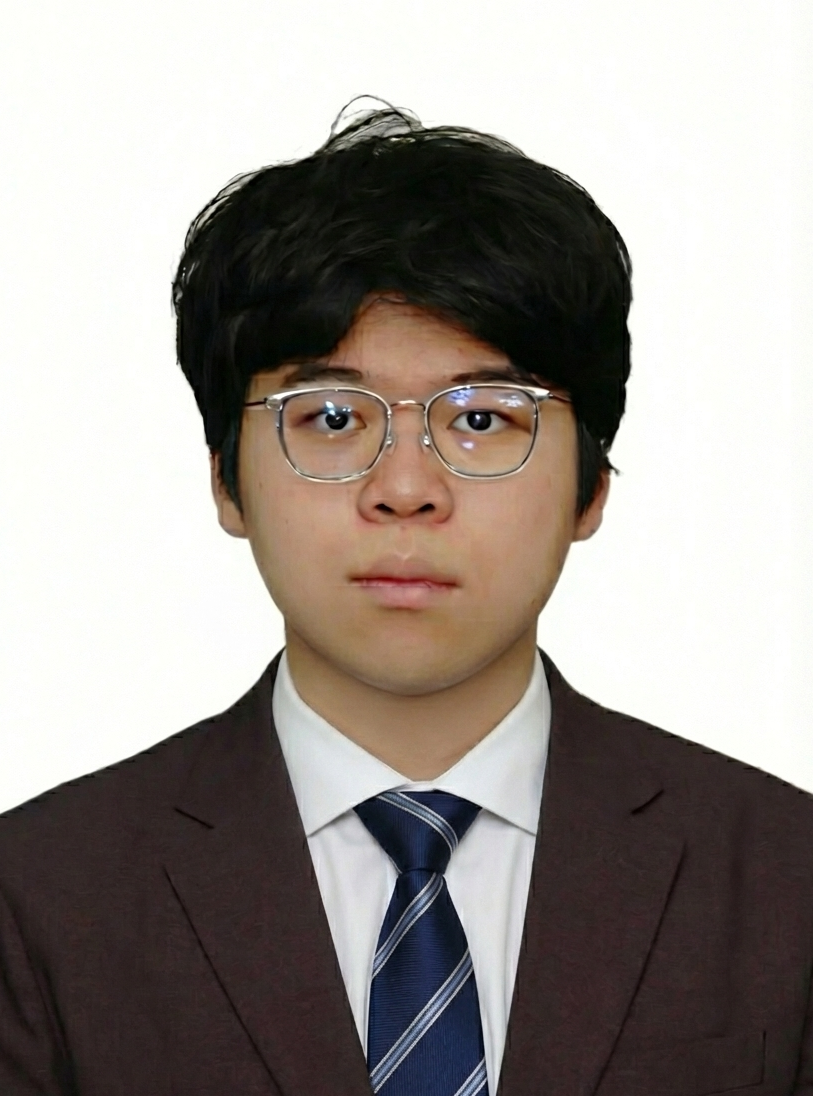
\includegraphics[width=3.2cm, height=4cm]{photo.png}
\end{minipage}

\vspace{8pt}

\section{教育背景}
\textbf{吉林大学 (Jilin University)} \hfill 2023.09 -- 至今 \\
唐敖庆理科试验班（生物方向），本科 \hfill 吉林，长春 \\
\begin{itemize}[noitemsep, topsep=2pt]
    \item \textbf{加权均分：} 88.44 / 100
    \item \textbf{GPA：} 3.59
    \item \textbf{英语水平：} IELTS: 6.0 | CET-4: 563 | CET-6: 461
    \item \textbf{核心课程：} Python程序设计基础(拔尖) 93.6、生物学创新创业实践 92、合成生物学 91、化学生物学 91、神经生物学 97、遗传学A 91.3、生物化学实验 94、无机化学实验 90.8、分析化学实验 92、物理化学实验 91.4、细胞生物学实验 94、微生物学实验 92、微积分A3 86.5
    \item \textbf{团支部书记} | 唐敖庆理科试验班 \hfill 2024 -- 至今
    \item \textbf{委员处委员} | 吉林大学学生代表大会 \hfill 2025 -- 至今
\end{itemize}

\section{学术成果 (Publications)}
目前已在 \textbf{JCIM, JPCB, IJMS} 等期刊发表学术论文共 \textbf{6} 篇，其中以第一作者身份发表两篇，部分代表作如下：
\begin{enumerate}
    \item \textbf{Qizheng He}, et al. "SRMMP-CharQM, Physics-Informed Deep Learning for Toxicity Prediction: Quantum Mechanical Descriptors Enable Scaffold Hopping in Mitochondrial Membrane Potential Assays." \textit{The Journal of Physical Chemistry B}, 2026.（第一作者）
    \item Huizi Cui, \textbf{Qizheng He}, et al. "Computational Insights into Reproductive Toxicity: Clustering, Mechanism Analysis, and Predictive Models." \textit{International Journal of Molecular Sciences}, 2024.（共同一作）
    \item Renxiu Song, Kaifeng Liu, \textbf{Qizheng He}, et al. "Exploring Bitter and Sweet: The Application of Large Language Models in Molecular Taste Prediction." \textit{Journal of Chemical Information and Modeling}, 2024.
\end{enumerate}

\section{荣誉奖项}
\begin{itemize}[noitemsep, topsep=2pt]
    \item {大学生创新创业训练计划 (大创) 省级优秀结题} \hfill 2026
    \item 吉林大学唐敖庆班科研实践奖学金 二等奖 \hfill 2025
    \item 吉林大学三等奖学金 \hfill 2024
    \item 吉林大学拔尖新生奖学金 \hfill 2023
    \item 全国中学生生物学竞赛 (CNBO) 铜牌 \hfill 2022
    \item 美国信息学奥林匹克竞赛 (USACO) Gold组 \hfill 2020
\end{itemize}

\section{实践经历}
\begin{itemize}[noitemsep, topsep=2pt]
    \item \textbf{BIOMOD世界总决赛}  作为主办方筹备工作，主管竞赛主会场 \hfill 2025.10
    \item \textbf{曼彻斯特大学 (University of Manchester)} 生命科学暑期学校 \hfill 2025.08
    \item \textbf{长白山野外实习} \hfill 2025.07
    \item \textbf{全国生物学拔尖基地云南高原植物勘察野外实习 (云南大学)} \hfill 2024.07
    \item \textbf{名校交流：} 牛津大学《神经生物学》(97分)；帝国理工学院《合成生物学》(91分)
\end{itemize}
\end{document}